%*****************************************
\chapter{Convolutional neural networks}\label{ch:conv_nets}
%*****************************************

\textbf{Convolutional Neural Networks} (\acsp{CNN}) are a kind of artificial feed-forward neural network in which the organization of the connections between the neurons is inspired by the animal visual cortex. Actually, individual cortical neurons respond to stimuli in a restricted region of space known as the \textbf{receptive field}. The receptive fields of different neurons partially overlap such that they tile the visual field. Similarly, in \acsp{CNN} each neuron is connected with only a small subset of inputs from the previous layer.

These networks are extremely useful when dealing with data with a grid-like topology, such as time-series data or images.

The name "convolutional neural network" indicates that the network employs a specialized kind of linear operation called \textbf{convolution}. In short, as stated in [\cite{Goodfellow-et-al-2016}], \emph{convolutional networks are simply neural networks that use convolution in place of general matrix multiplication in at least one of their layers}.

\section{Main features}

While traditional \acf{MLP} models were successfully used in the past for image recognition, due to the full connectivity between nodes they suffer from the curse of dimensionality and thus do not scale well to higher resolution images.

For instance, in the CIFAR-10 dataset, images are of size $32x32x3$ (32 wide, 32 high, 3 color channels), so a single fully connected neuron in the first hidden layer of a regular \ac{MLP} would have $32*32*3 = 3,072$ weights. A $200x200$ image, however, would lead to neurons that have $200*200*3 = 120,000$ weights.
Such network architecture does not take into account the spatial structure of data, treating input pixels which are far apart or close together exactly in the same way. The full connectivity of neurons is wasteful in the framework of image recognition, and the huge number of parameters quickly leads to overfitting.

As said before, convolutional neural networks are biologically inspired variants of multilayer perceptrons, designed to emulate the behaviour of a visual cortex. These models mitigate the challenges posed by the \ac{MLP} architecture by exploiting the strong spatially local correlation present in natural images.
In particular, \acsp{CNN} have the following distinguishing features:

\begin{description}
	
	\begin{figure}
		\centering
		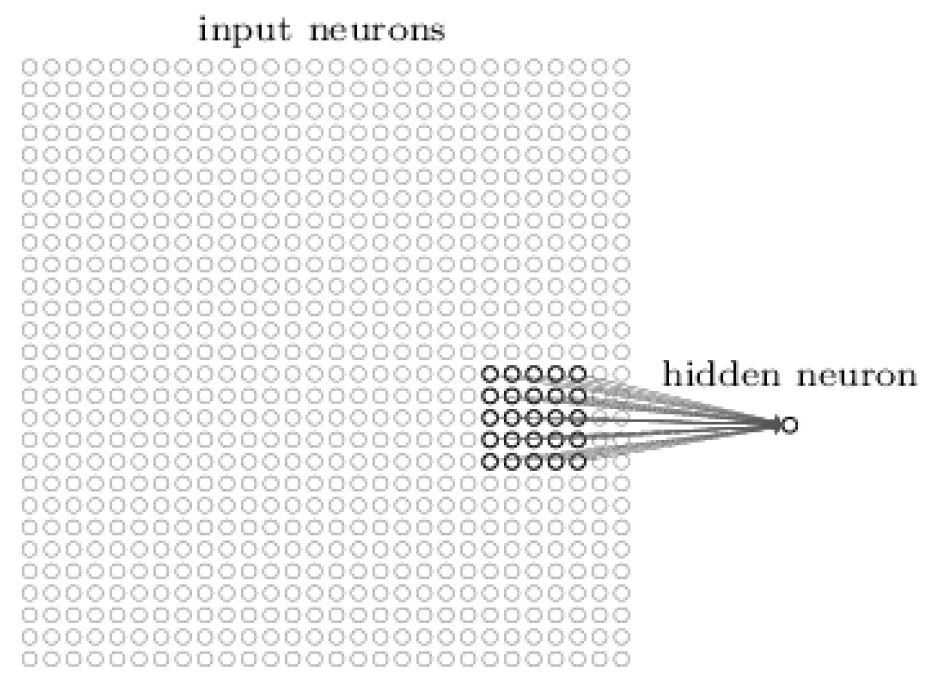
\includegraphics[width=0.7\textwidth]{Images/receptive_field}
		\caption{Implementation of a $5x5$ receptive field in a \acs{CNN}}\label{fig:receptive_field}
	\end{figure}
	
	\item[3D volumes of neurons] The layers of a \acs{CNN} have neurons arranged in 3 dimensions: width, height and depth. Neurons inside a layer are only connected to a small region of the layer before it, called a receptive field. Figure \ref{fig:receptive_field}, for instance, shows a $5x5$ receptive field from the input neurons to the first hidden layer, with a $28x28$ input. Distinct types of layers, both locally and completely connected, are stacked to form the \acs{CNN} architecture.
	
	\item[Local connectivity] Following the concept of receptive field, \acsp{CNN} exploit spatially local correlation by enforcing a local connectivity pattern between neurons of adjacent layers. The architecture thus ensures that every \textbf{filter} (\ie weight patch) learnt produces the strongest response to a spatially local input pattern. Stacking many of such layers leads to non-linear filters that become increasingly "global" (\ie responsive to a larger region of input space). This allows the network to first create good representations of small parts of the input, then assemble representations of larger areas from them.
	
	\item[Shared weights] In \acsp{CNN}, each filter is replicated across the entire visual field. These replicated units share the same parameterization (weight vector and bias) and form a feature map. This means that all the neurons in a given convolutional layer detect exactly the same features. Replicating units in this way allows for features to be detected regardless of their position in the visual field, thus constituting the property of translation invariance.
	
\end{description}

Together, these properties allow convolutional neural networks to achieve better generalization performances in vision problems. Moreover, th weight sharing helps by dramatically reducing the number of free parameters being learnt, thus lowering the memory requirements for running the network. Decreasing the memory footprint allows the training of larger, more powerful networks.

\begin{figure}
	\centering
	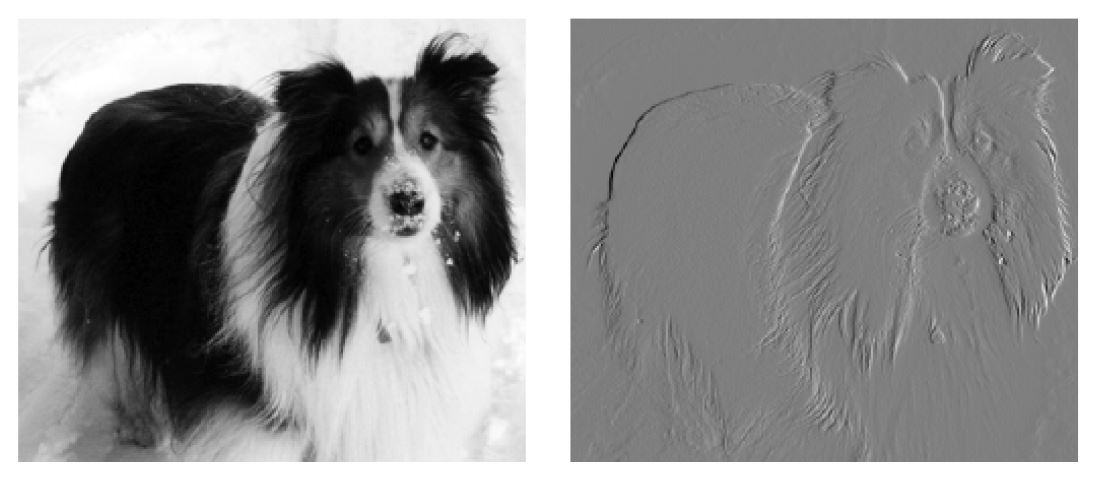
\includegraphics[width=0.7\textwidth]{Images/filter_application}
	\caption{Application of a filter for edge detection (Photo credit: Paula
		Goodfellow)}\label{fig:filter_application}
\end{figure}

The output of a convolutional layer, \ie the the matrix formed by sliding a given filter over the input and and computing the dot product, is called \textbf{feature map}. It is evident that different filters will produce different feature maps for the same input. Figure \ref{fig:filter_application} shows the result of the application of a filter for edge detection to a given image. The image on the right was formed by taking
each pixel in the original image and subtracting the value of its neighboring pixel on the left. This shows the strength of all of the vertically oriented edges in the input image,
which can be a useful operation for object detection.

In order to recognize an image, we'll need more than one filter. For this reason, the output of a full convolutional layer will be a set of feature maps with the following structure:

\begin{figure}[h]
	\centering
	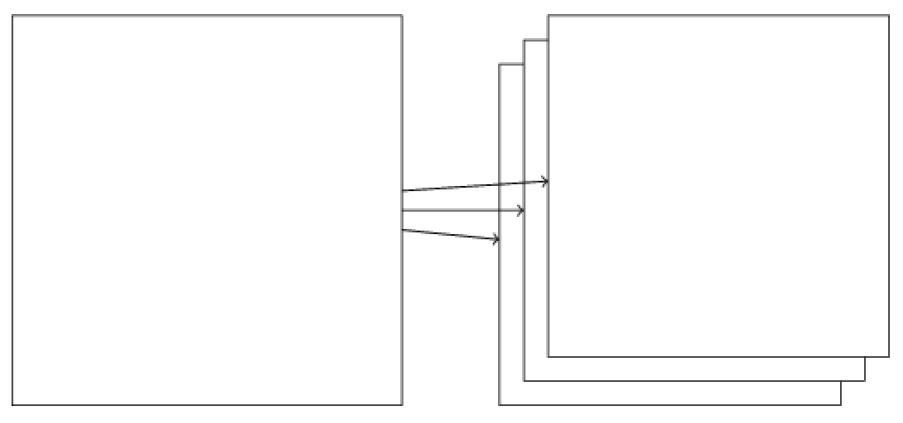
\includegraphics[width=0.7\textwidth]{Images/feature_maps}
	\caption{Application of three filters to a given input producing three different feature maps}\label{fig:feature_maps}
\end{figure}

The amount by which the filter shifts is called \textbf{stride} and it controls how the filter convolves around the input volume.

\begin{figure}[h]
	\centering
	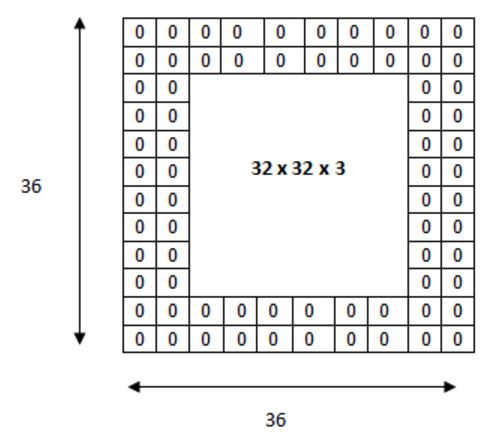
\includegraphics[width=0.7\textwidth]{Images/zero_padding}
	\caption{Zero padding of two applied to a $32x32x3$ picture}\label{fig:zero_padding}
\end{figure}

In order to have an output of the same size of the input, it is necessary to add some additional pixels to the input image, this is called \textbf{padding}. For instance, a zero padding like the one in figure \ref{fig:zero_padding} pads the input volume with zeros all around the border.

In general, the formula for calculating the output size for any given convolutional layer is:

\begin{equation} \notag
	O=\frac{W-K+2P}{S}+1
\end{equation}
where O is the output height/length, W is the input height/length, K is the filter size, P is the padding, and S is the stride.
